% !TEX root = ../Thesis.tex
%%
%%  Hochschule für Technik und Wirtschaft Berlin --  Abschlussarbeit
%%
%% Kapitel 2 - Theoretische Grundlagen und Forschungsstand
%%
%%


\chapter{Theoretische Grundlagen und Forschungsstand} \label{Grundlagen}

In diesem Kapitel werden die nötigen Grundlagen zum Verständnis des Portscanning in Form von SYN-Scans, sowie 
das nötige Wissen über Netzwerkkommunikation, die genutzten Technologien und Linux-Schnittstellen vermittelt.
Des Weiteren wird auf Asynchrone Programmierung eingegangen, sodass ein Verständnis für das nachfolgende Konzept 
der Implementierung gegeben ist.

Anschließend werden die zum Vergleich genutzten Scanner vorgestellt und eingeordnet. Auch Rust und dessen 
Besonderheiten wird genauer vorgestellt.

\section{Grundlagen der Netzwerkkommunikation}
Bei der Kommunikation in TCP/IP \footnote{Eine grundlegende Kenntnis über das TCP/IP Modell wird angenommen} Netzwerken dient das IP-Protokoll und die IP-Adressen zur Identifikation der Maschine im Netzwerk, während die genaue 
Adressierung der spezifischen Anwendungen durch sogenannte Ports bzw. der sogenannten Portnummer bestimmt wird \cite{Lyon_2010} (TODO SEITE?). 
Die Portnummer ist ein 16-Bit-Wert und kann somit zwischen jeweils einschließlich 0 und 65535 liegen [Computernetzwerke S107]. Einige Portnummern
sind fest vergeben oder für bestimmte Anwendungen registriert \cite{IANA_Port_Registry}, was es ermöglicht, gezielt nach bestimmten Anwendungen zu scannen.

\subsection{Ports}
Ports können in verschiedene Zustände eingeordnet werden. Für diese Arbeit ist nur die Unterscheidung zwischen offen und geschlossen/gefiltert relevant.

Offen: Eine Anwendung lauscht auf dem Port und akzeptiert eingehende valide TCP oder UDP Anfragen \cite{Lyon_2010}.
Geschlossen / Gefiltert: Der mit dem Port verbundene Service ist zwar ansprechbar, aber akzeptiert keine eingehenden Verbindungen / 
Es gibt lediglich eine ICMP (Fehler) Antwort oder gar keine, da beispielsweise kein Service für diesen Port
existiert \cite{Lyon_2010}.

Ein IP-Port Paar z.B. 192.178.0.42:8080 wird Socket bzw. Socket Paar genannt. 

mglw. Irrelevant: Ein Verbindung zweier Rechner über einen spezifischen Dienst ist durch die beiden
Socket Paare eindeutig identifizierbar [Computernetzwerke S108]. 

\subsection{Transmission Control Protocol (TCP)}
Das Transmission Control Protocol operiert in der Transportschicht des TCP/IP Modells und ist eines der meistgenutzten
Transportprotokoll des Internets \cite{Wendzel_2021} TODO S71. Es gewährleistet eine zuverlässige, verbindungsorientierte
Datenübertragung zwischen den Prozessen der Hosts. Die ursprüngliche Spezifikation erfolgte im RFC 793 \cite{Postel_1981},
welches durch RFC 9293 \cite{Eddy_2022} konsolidiert wurde. Für die Entwicklung eines SYN-Portscanners sind insbesondere
der Aufbau des TCP-Headers und der Mechanismus des Verbindungsaufbaues entscheidend. 


Da das TCP Protokoll Daten 
als Datenstrom (Stream) statt einzeln (Message) versendet, wird vorher eine Verbindung in einem sogenannten 
\textit{Three-Way-Handshake} aufgebaut \cite{Wendzel_2021} S71/72. Bei diesem werden TCP Pakete mit jeweils unterschiedlichen
Werten in den \textit{Control Bits (Flags)} des TCP-Headers nach folgendem Muster ausgetauscht:

\begin{figure}[htbp]
	\centering
	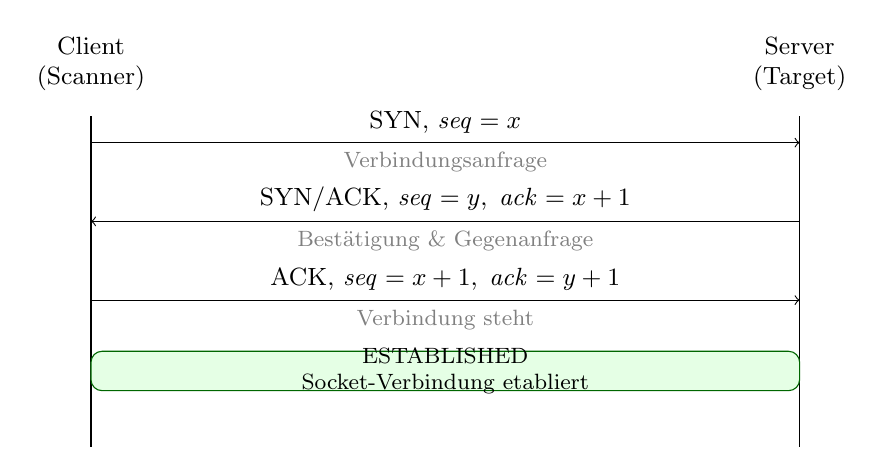
\begin{tikzpicture}[font=\small]
		\node[align=center] (c) at (0,0) {Client\\(Scanner)};
		\node[align=center] (s) at (9,0) {Server\\(Target)};

		\draw (c.south) ++(0,-0.2) -- ++(0,-4.2);
		\draw (s.south) ++(0,-0.2) -- ++(0,-4.2);

		\draw[->] (0,-1.0) -- node[above] {SYN, $\mathit{seq}=x$} node[below, font=\footnotesize, text=gray] {Verbindungsanfrage} (9,-1.0);
		\draw[->] (9,-2.0) -- node[above] {SYN/ACK, $\mathit{seq}=y,\; \mathit{ack}=x+1$} node[below, font=\footnotesize, text=gray] {Bestätigung \& Gegenanfrage} (0,-2.0);
		\draw[->] (0,-3.0) -- node[above] {ACK, $\mathit{seq}=x+1,\; \mathit{ack}=y+1$} node[below, font=\footnotesize, text=gray] {Verbindung steht} (9,-3.0);

		\draw[rounded corners, fill=green!10, draw=green!40!black] (0,-3.65) rectangle (9,-4.15);
		\node[align=center, font=\footnotesize] at (4.5,-3.9) {ESTABLISHED\\Socket-Verbindung etabliert};
	\end{tikzpicture}
	\caption{Der TCP Three-Way-Handshake. Entscheidend für die Zuordnung ist, dass die \textit{Acknowledgment Number} im zweiten Schritt dem Wert der initialen \textit{Sequence Number} + 1 entspricht ($x+1$).}
	\label{fig:handshake_detail}
\end{figure}

Da das TCP Protokoll Daten als Datenstrom (Stream) statt einzeln (Message) versendet, 
wird vorher eine Verbindung in einem sogenannten \textit{Three-Way-Handshake} aufgebaut \cite{Wendzel_2021} S71/72. 
Bei diesem werden TCP Pakete mit jeweils unterschiedlichen Werten in den \textit{Control Bits (Flags)} 
des TCP-Headers nach folgendem Muster ausgetauscht:

\begin{figure}[htbp]
	\centering
	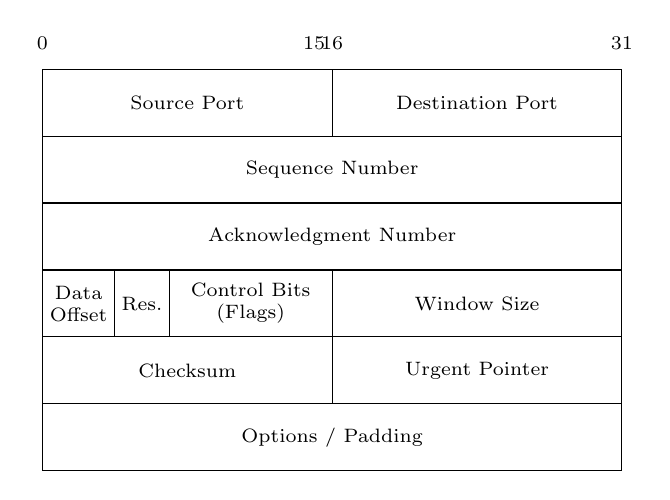
\begin{tikzpicture}[x=0.23cm, y=0.85cm, every node/.style={font=\scriptsize, align=center}]
		% Bit indices
		\node[anchor=south] at (0,6.15) {0};
		\node[anchor=south] at (16,6.15) {16};
		\node[anchor=south] at (32,6.15) {31};
		\node[anchor=south] at (15,6.15) {15};

		% Row 1
		\draw (0,6) rectangle (16,5) node[midway] {Source Port};
		\draw (16,6) rectangle (32,5) node[midway] {Destination Port};

		% Row 2
		\draw (0,5) rectangle (32,4) node[midway] {Sequence Number};

		% Row 3
		\draw (0,4) rectangle (32,3) node[midway] {Acknowledgment Number};

		% Row 4
		\draw (0,3) rectangle (4,2) node[midway] {Data\\Offset};
		\draw (4,3) rectangle (7,2) node[midway] {Res.};
		\draw (7,3) rectangle (16,2) node[midway] {Control Bits\\(Flags)};
		\draw (16,3) rectangle (32,2) node[midway] {Window Size};

		% Row 5
		\draw (0,2) rectangle (16,1) node[midway] {Checksum};
		\draw (16,2) rectangle (32,1) node[midway] {Urgent Pointer};

		% Row 6
		\draw (0,1) rectangle (32,0) node[midway] {Options / Padding};
	\end{tikzpicture}
	\caption{Aufbau des TCP-Headers (ohne Nutzdaten). Für SYN-Scans sind insbesondere die \textit{Control Bits} (z.\,B. SYN, RST, ACK) relevant.}
	\label{fig:tcp_header}
\end{figure}


\section{Portscanning}
Portscanning, als Art des Netzwerkscannings, ist eines der fundamentalen Verfahren in der Netzwerksicherheit zum Auffinden von 
potentiellen Schwachstellen \cite{Lyon_2010}. Ein Portscanner verschickt Pakete an ein Zielsystem und
zieht anhand der Antworten, oder auch ausbleibenden Antworten, Rückschlüsse auf den Zustand des Systems. Das Ziel ist die Identifikation
von offenen Ports bzw. aktiven Diensten, was als erster Schritt für weiterführende Sicherheitsanalysen oder aber auch Angriffe dienen kann. [TODO NIST S4-3] 

Beim Scannen von Ports können grundsätzlich zwei strategische Ausrichtungen unterschieden werden:
- Vertikales Scannen: Hierbei wird ein einzelner Ziel-Host (TODO Host erklären) auf eine Vielzahl von Ports (oft alle 65535) gescannt, um ein möglichst
vollständiges Profil möglicher Schwachstellen des Zielsystemes zu erlangen und somit eher für das Penetrationtesting geeignet ist.
- Horizontales Scannen: Ein sehr großer Addressbereich, beispielsweise das komplette IPv4-Internet wird gescannt. Dafür ist die Anzahl
der zu scannenden Ports sehr klein oder auf einen einzigen beschränkt. Dies bietet die Möglichkeit wertvolle Daten über Trends oder
die Verbreitung von Schwachstellen zu untersuchen \cite{Durumeric_Wustrow_Halderman}.

\subsection{SYN-Scanning}
Für einen \textit{half-open} SYN-Scan wie er in dieser Arbeit behandelt wird, sind lediglich die ersten beiden Schritte des Verbindungsablaufes
relevant. Es wird davon gebraucht gemacht, dass bereits und ausschließlich eine SYN/ACK Antwort den Port als offen klassifiziert, 
was den weiteren Verbindungsaufbau irrelevant macht \cite{Lyon_2010}. Um den Scan zu verschleiern und den Verbindungsversuch trotz dessen sauber
abzuschießen, kann anschließend noch ein Paket, bei welchem die RST Flag der Control Bits gesetzt ist gesendet werden \cite{Lyon_2010}.

Um antwortende Hosts effizient zu identifizieren, wird das Prinzip des SYN-Cookies adaptiert, welches ursprünglich als 
Abwehrmechanismus gegen Denial-of-Service-Angriffe spezifiziert wurde \cite[S. 8]{Eddy_2007}. Dieses Verfahren bietet den Vorteil, 
dass der Scanner keinen Zustand für die versendeten Pakete im Arbeitsspeicher halten muss. Stattdessen werden verbindungsspezifische 
Informationen unter Verwendung eines Hash-Algorithmus (z. B. keyed SipHash) kodiert 
und als \textit{Sequence Number} in den TCP-Header des ausgehenden SYN-Pakets eingetragen.
Antwortet ein Ziel-Host mit einem SYN-ACK-Paket, so enthält dessen Acknowledgment Number gemäß TCP-Spezifikation den inkrementierten 
Wert der ursprünglichen \textit{Sequence Number}. Die Validierung lässt sich abstrahiert wie folgt beschreiben:

\begin{verbatim}is_valid = hash(value_0, value_1, ..., secret) == answer.ack_num - 1\end{verbatim}

Entscheidend für den Scanner sind also folgende Header Felder: 

\begin{table}[htbp]
\caption{TCP Header Felder}
\resizebox{\textwidth}{!}{
\begin{tabular}{|c|c|}\hline
\textbf{Header Feld} & \textbf{Beschreibung} \\ \hline
Source Port & Beschreibt den genutzten Port des Ausgangsdienstes. \\ \hline
Destination Port &  Beschreibt den zu scannenden Port des Zielsystems. \\ \hline
Sequence Number & Wird zur Speicherung des SYN-Cookies genutzt. \\ \hline
Acknowledgement Number & Wird zum Abrufen des SYN-Cookies genutzt. \\ \hline
Control Bits (Flags) & Wird für die verschiedenen Phasen des Verbindungsaufbaues angepasst oder ausgelesen.  \\ \hline
\end{tabular}
}
\label{tab:TCP-header-fields}
\end{table}

\section{Schnittstellen zur Paketverarbeitung unter Linux}
Um einen performanten Scanner zu bauen, müssen die genutzten Technologien zum einen für die Netzwerkprogrammierung 
geeignet und zum anderen hohe Sende- und Empfangsraten zulassen, während möglichst wenig
Rechenressourcen verbraucht werden. 

\subsection{Linux}
Linux ist ein Open-Source Betriebssystem-Kernel, welcher aufgrund neuartiger Subsysteme (wie eBPF [später] und XDP [später]), eine 
programmierbare Paketverarbeitung nahe an der Hardware ermöglicht \cite{Kerrisk_2018}. Dies ist für die Entwicklung eines Hochleistungs-Scanners
von großem Vorteil.

Ein zentrales Konzept zum Verständnis der Performance-Grenzen ist die Unterscheidung 
zwischen \textit{User Space} und \textit{Kernel Space} \cite{Kerrisk_2018} S23: 

\begin{itemize} 
	\itemsep 0pt
	\item \textbf{Kernel Space:} Hier läuft der Kern des Betriebssystems (Ring 0) mit vollem Zugriff 
	auf die Hardware und den Speicher. Treiber und der Netzwerk-Stack operieren auf dieser Ebene. 
	\item \textbf{User Space:} Hier laufen reguläre Anwendungen (Ring 3) in isolierten Speicherbereichen. 
\end{itemize} 
Die Kommunikation zwischen diesen Ebenen erfolgt über \textit{System Calls}. Jeder Wechsel (\textit{Context Switch}) 
zwischen User und Kernel Space, sowie das Kopieren von Daten zwischen diesen 
Speicherbereichen, erzeugt Overhead. Beim Versenden und Empfangen sehr vieler Pakete 
summiert sich dieser Overhead, da jedes Paket im Normalfall sowohl Kernel Space, als auch User Space, durchschreitet [TODO].
Dies belastet die CPU und wird für den Durchsatz zum Flaschenhals.

\subsection{Raw-Sockets und Address Families}
Als Endpunkt für die Kommunikation werden \textit{Sockets} genutzt \cite{socket2_linux_manpage}. Die traditionelle 
Netzwerkprogrammierung unter Linux abstrahiert die Komplexität der Netzwerkprotokolle wie TCP. So übernimmt der Kernel
dabei vollständig den \textit{Three-Way-Handshake} und das Zustandsverwaltung [TODO]. 
Für einen SYN-Scanner ist dies ungeeignet, da der Scanner lediglich das initiale SYN-Paket senden und die Antwort 
registrieren will, ohne eine vollwertige Verbindung aufzubauen, welche Ressourcen im Kernel binden würde.

RAW Sockets erlauben der Anwendung, Netzwerkpakete unter Umgehung bestimmter Layer des Kernel-Stacks zu senden 
und zu empfangen \cite{raw7_linux_manpage}. Der Entwickler muss die Protokoll-Header selbst konstruieren. 
Dies ist für half-open Port-Scanner essenziell, um individuelle Pakete zu generieren, ohne dass der Kernel 
automatisch in den Verbindungsaufbau eingreift. 

Die Adress-Familien definieren dabei die Interpretation der Adressen und die Ebene des Zugriffs \cite{address_families7_linux_manpage}. 
Hier ein paar Beispiele: TODO Besser formulieren
\begin{itemize} 
	\itemsep 0pt
	\item \textbf{AF\_INET (Standard):} AF\_INET Operiert auf Layer 3 (IP Ebene), deshalb fügt der Kernel den IP-Header hinzu. 	
	Auch das Routing wird (TODO vollständig?) durch den Kernel vorgenommen. 
 	\item \textbf{AF\_PACKET (Performant):} Diese Familie ermöglicht direkten Zugriff auf Layer 2 (Ethernet-Ebene). 
	Anwendungen können rohe Ethernet-Frames lesen und schreiben. Dies bietet die vollständige Kontrolle
	über die Paketerstellung. TODO wie weit durch Kernel geschickt? 
	\item \textbf{AF\_XDP (Sehr Performant):} Hierbei handelt es sich um eine für Hochleistungspaketverarbeitung optimierte Address-Familie. 
	Sie ermöglicht das Senden und Empfangen von Paketen unter fast vollständiger Umgehung des Kernel-Stacks. 
\end{itemize}

(TOOD -> Abbildung Netzwerkstack bzw Paketverlauf)

\subsection{Erweiterte Berkley Packet Filter (eBPF)}
Ursprünglich als \textit{Berkeley Packet Filter} (BPF) für Werkzeuge wie tcpdump entwickelt, um Pakete effizient zu filtern \cite{260309}, 
wurde die Technologie zum erweitert, sodass grundlegend neue Möglichkeiten erschlossen wurden. 

eBPF ist eine im Linux-Kernel integrierte virtuelle Maschine (VM), die es erlaubt, benutzerdefinierten 
Bytecode sicher und effizient im Kernel-Kontext auszuführen, ohne Kernel-Module schreiben oder den Kernel 
neu kompilieren zu müssen \cite{Nishanth_Reddy_Pinnapareddy_2025} S207. eBPF-Programme werden zur Laufzeit 
durch einen JIT-Compiler (Just-In-Time) in native Maschinensprache übersetzt. Ein \textit{Verifier} stellt 
vor der Ausführung sicher, dass der Code sicher ist TODO cite. 
So werden Fehler wie beispielsweise Endlosschleifen oder falsche Speicherzugriffe vermieden.

Für einen SYN-Scanner ist eBPF nützlich, da es ermöglicht, eingehende Antwortpakete (SYN-ACK) extrem früh 
zu filtern und an den User Space weiterzuleiten, bevor teure Speicherstrukturen des Kernels angelegt werden. 
So werden nur relevante Daten an den User Space weitergereicht. 

\subsection{eXpress Data Path (XDP)} 
XDP definiert eine limitierte Ausführungsumgebung für eBPF-Programme, die direkt im Kontext des 
Netzwerktreibers ausgeführt werden.
Dies ermöglicht eine programmierbare Hochleistungspaketverarbeitung direkt im Betriebssystemkern. 
Im Gegensatz zu früheren Ansätzen, die den Kernel vollständig umgehen (z.B. DPDK), 
integriert sich XDP kooperativ in den bestehenden Stack \cite{Høiland-Jørgensen_Brouer_Borkmann_Fastabend_Herbert_Ahern_Miller_2018}. 

Ein XDP-Programm kann Pakete verwerfen (XDP\_DROP), an den regulären Netzwerkstack weiterleiten (XDP\_PASS), 
über dieselbe Schnittstelle zurücksenden (XDP\_TX) oder an eine andere CPU bzw. einen Userspace-Socket 
umleiten (XDP\_REDIRECT) \cite{Høiland-Jørgensen_Brouer_Borkmann_Fastabend_Herbert_Ahern_Miller_2018}\cite{Vieira_Castanho_Pacífico_Santos_Júnior_Vieira_2021}.

Die Effizienz von XDP resultiert aus der Positionierung im Datenpfad. In herkömmlichen 
Linux-Netzwerkarchitekturen durchläuft ein Paket nach dem Empfang durch die Netzwerkkarte (NIC) den 
gesamten Netzwerk-Stack. Erst danach erreichen die Daten den User Space. Dies erfordert CPU und Speicher-
aufwendige Kontextwechsel (Context Switches) zwischen Kernel- und User-Mode, sowie die Allokation 
komplexer Metadatenstrukturen (sk\_buff) (TODO siehe Abbildung vorher) \cite{Høiland-Jørgensen_Brouer_Borkmann_Fastabend_Herbert_Ahern_Miller_2018}\cite{Zhang_Shu_Chen_Xie_2024}.

XDP greift vor dieser Allokation ein (TODO siehe Abbildung). Tests zeigen, dass XDP auf einem einzelnen CPU-Kern bis zu 
fünfmal mehr Pakete pro Sekunde verarbeiten kann als der Standard Linux-Stack \cite{Høiland-Jørgensen_Brouer_Borkmann_Fastabend_Herbert_Ahern_Miller_2018}.

-> Abbbildung XDP einfügen

Die Performance und Verfügbarkeit von XDP hängen vom verwendeten Betriebsmodus ab. 
Nach Zhang et al. \cite{Zhang_Shu_Chen_Xie_2024} und Vieira et al. \cite{Vieira_Castanho_Pacífico_Santos_Júnior_Vieira_2021} 
lassen sich drei Modi unterscheiden:

\begin{itemize} 
	\item \textbf{Native Mode (Driver Mode):} Dies ist der Standardmodus für Hochleistungsanwendungen. 
	Das XDP-Programm wird direkt im Netzwerkkartentreiber ausgeführt. Die Verarbeitung erfolgt nach dem 
	DMA-Transfer (Direct Memory Access) in den Ring-Buffer, aber vor der sk\_buff-Allokation. 
	Dies erfordert explizite Unterstützung durch den Treiber der Netzwerkkarte. 
	\item \textbf{Offloaded Mode (Hardware Mode):} Hierbei wird das eBPF-Programm vom Kernel auf die 
	Netzwerkkarte ausgelagert und direkt auf der Hardware ausgeführt. Dies bietet die höchste 
	Performance, da die Host-CPU vollständig von der Paketverarbeitung entlastet wird, setzt aber
	die Nutzung einer sogenannten \textit{Smart NIC} Netzwerkkarte voraus. 
	\item \textbf{Generic Mode (SKB Mode):} Dieser Modus dient der Kompatibilität. Wenn ein Treiber XDP 
	nicht nativ unterstützt, führt der Kernel das XDP-Programm an einer späteren Stelle im Netzwerkstack 
	aus. Zwar gehen hier die massiven Performance-Vorteile der Speicherersparnis verloren, 
	jedoch wird sichergestellt, dass XDP-Anwendungen auf jeder Hardware funktionsfähig bleiben. 
	Trotzdem profitiert es von effizienteren, sperrfreien Ring-Buffer-Strukturen (<- TODO bessere Argumente)
\end{itemize}


\section{Abgrenzung des Themas} \label{Abgrenzung}

. Außerdem ist es das Ziel, horizontal (TODO siehe nächstes Kapitel) zu scannen. Anders als 
beispielsweise der reguläre SYN-Scan des Tools NMap \cite{Lyon_2010}, welcher in der Regel vertikal erfolgt.

Mechanismen zur Erkennungsvermeidung des Scans werden in dieser Implementierung nur rudimentär behandelt, da der Fokus
klar auf der Performance und Ressourceneffizienz der Anwendung liegt. 
Außerdem beschränkt sich diese Arbeit auf den IPv4 Addressraum, da dies genügt, um der Forschungsfrage nachzugehen.




















%%
%% Alt
%%

\begin{table}[htbp]
\caption{OSI-7-Schichtenmodell}
\resizebox{\textwidth}{!}{
\begin{tabular}{|c|c|c|c|c|}\hline
  \multicolumn{3}{|c|}{\textbf{Schicht}} & \textbf{Beispielprotokoll} & \textbf{TCP/IP-Modell} \\ \hline
  7 & Anwendungsschicht & Application Layer & \multirow{3}{*}{HTTP, FTP, SNMP} & \multirow{3}{*}{Application Layer} \\ \cline{1-3}
  6 & Darstellungsschicht & Presentation Layer & & \\ \cline{1-3}
  5 & Sitzungsschicht & Session Layer & & \\ \hline
  4 & Transportschicht & Transport Layer & TCP, UDP & Transport Layer \\ \hline
  3 & Vermittlungsschicht & Networking Layer & IPv4, IPv6, ICMP & Internet Layer \\ \hline
  2 & Sicherungsschicht & Data Link Layer & \multirow{2}{*}{Ethernet, WLAN, ISDN} & \multirow{2}{*}{Link Layer} \\ \cline{1-3}
  1 & Physikalische Schicht & Physical Layer & & \\ \hline
\end{tabular}
}
\label{tab:OSI-7-Schichtenmodell}
\end{table}

\begin{figure}[htbp]
	\centering
	\includegraphics[width=12cm]{wireless_sensor_network}
	\caption{Aufbau eines drahtlosen Sensornetzwerkes}
	\label{fig:wsn}
\end{figure}

Bei drahtlosen Sensornetzen, international auch Wireless Sensor Networks (WSN) genannt, handelt es sich um Netzwerke aus kleinen Sensoren, die ihre Messergebnisse zu einer zentralen Station senden. Die Sensoren helfen dabei einander, die Informationen weiterzureichen (siehe Abbildung \ref{fig:wsn}). So ein drahtloses Sensornetz kann zum Beispiel in einem Gebäude Temperatur- und Luftfeuchtigkeitswerte an eine zentrale Station liefern, die dann die Klimaanlage entsprechend ansteuert. Eine komplette Verkabelung jedes einzelnen Sensors kann dabei je nach Anzahl sehr aufwendig und kostspielig sein. Wenn die Sensoren dazu noch mobil sein sollen, empfiehlt sich eine drahtlose Kommunikation.

Ein Sensor in einem drahtlosen Sensornetz ist ausgestattet mit einer Kommunikationseinheit, die sich selbstständig innerhalb des Netzes konfiguriert und darüber die eingelesenen Messgrößen zu einer zentralen Stelle transportiert.

%%Ein Sensor ist dabei ein typisches Smart Object. Es 
%% Das Steuergerät soll dabei möglichst klein sein, damit es in einem Steckdosengehäuse Platz finden kann. 
%% Der Fernzugriff soll mithilfe des Protokolls IPv6 erfolgen, um zukunftssicher auf die Infrastruktur des Internet verwenden zu können. 

\subsection{Smart Objects}\label{Smart Objects}

Diese Definition von Smart Objects \index{Smart Object} beruht auf \textcite{vasseur10interconnecting}. Dabei handelt es sich um kleine Objekte, die mit folgenden Einheiten ausgestattet sind:

\begin{itemize}
	\itemsep 0pt
	\item eine Form von Sensor und/oder Aktor
	\item ein kleiner Mikrocontroller
	\item eine Kommunikationseinheit
	\item eine Energieversorgung
\end{itemize}

Ein Sensor und/oder Aktor wird benötigt, um mit der Umwelt interagieren zu können. Ein Sensor kann bestimmte Messgrößen erfassen, die dann verarbeitet werden können. Ein Aktor ist das Gegenstück zu einem Sensor. Über ihn kann aktiv die Umwelt beeinflusst werden. Die Kommunikationseinheit befähigt das Smart Object über ein Netzwerk kommunizieren zu können. Es ist dabei möglich mit anderen Smart Objects zu kommunizieren als auch mit weit entfernten Geräten, im Falle des Internets weltweit. Ein kleiner Mikrocontroller übernimmt die Informationsverarbeitung. Dieser nimmt Daten von Sensoren entgegen bzw. steuert den Aktor. Die Kommunikation wird ebenso von ihm geregelt, von einem Sensor gemessene Werte können über das Netzwerk weitergegeben werden. Der Mikrocontroller kann als Kern des Smart Object angesehen werden. Die Energieversorgung ist notwendig, um alle Einheiten ausreichend mit elektrischer Energie zu versorgen.

Alle diese technischen Eigenschaften machen ein Objekt aber noch nicht zu einem Smart Object. Erst die Anwendung und sein Verhalten machen aus einem Objekt mit den obigen Eigenschaften ein Smart Object. Allerdings ist es sehr schwierig, dieses Verhalten zu definieren. Die Anwendungen sind sehr unterschiedlich und es ist völlig unbekannt, wie Smart Objects in der Zukunft eingesetzt werden. Gemeinsam ist allen Anwendungen allerdings, dass Smart Objects mit der physikalischen Umwelt interagieren und über ein Netzwerk kommunizieren. Dieses Verhalten und die obigen technischen Eigenschaften machen ein Smart Object aus.

Von der Kommunikationstechnologie her ähnelt ein Smart Object einem Sensor in einem Sensornetz. Allerdings ist im Gegensatz zu einem Sensornetz ein Netz aus Smart Objects nicht allein auf die Datenübermittlung fokussiert. Bei einem Sensornetz ist der Datenfluss immer vom Sensor ins Netzwerk, wohingegen der Datenfluss bei einem Smart Object bidirektional ist. Der Fokus liegt dabei auf eine Vielzahl von Funktionen insbesondere der Steuerung und Überwachung \citep[Seite 12]{vasseur10interconnecting}. Es ist also die Anwendung, die ein Gerät zu einem Smart Object macht. Aber Entwicklungen, hauptsächlich in der Energieversorgung und Kommunikationstechnik, kommen beiden Forschungsgebieten zugute.


\subsection{Internet-of-Things}

\begin{figure}[htbp]
	\centering
	\includegraphics{internet_of_things}
	\caption{Die Internet-of-Things Vision \cite[Figure 1.2]{Bormann:6LoWPAN}}
	\label{fig:internet_of_things}
\end{figure}

Das Internet-of-Things, auch Internet der Dinge genannt, ist eine Vision, wie sich das Internet in Zukunft entwickeln kann. Es soll aus der Vernetzung vieler Kleinstgeräte -- auch oder vielleicht hauptsächlich Smart Objects -- bestehen. \textcite{Bormann:6LoWPAN} betrachten das Internet-of-Things als eine weitere Schale des Internets (Abbildung \ref{fig:internet_of_things}), die gerade anfängt sich heraus zu bilden. Der Kern des Internets (Core Internet) besteht heute aus vielen Routern und Servern, die zusammen Millionen von Teilnehmern ausmachen. Um diesen Kern herum liegt das sogenannte Fringe Internet, was beispielsweise aus privaten Rechnern oder Laptops besteht, aber auch aus lokalen Netzwerken, die zum Internet verbunden werden. Die Teilnehmer des Fringe Internet gehen in die Milliarden. Um dieses Fringe Internet herum beginnt sich eine weitere Schale zu bilden, das sogenannte Internet-of-Things. Auf lange Sicht kann hier mit Billionen von Teilnehmern gerechnet werden. Hauptsächlich bestehen diese Teilnehmer aus IP-fähigen eingebetteten Systemen (embedded systems). Eine so große Zahl an Teilnehmern kann nur mithilfe des Internet Protokolls der Version 6 ans Internet angeschlossen werden, da das bisherige Internet Protokoll der Version 4 keine freien Adressräume mehr zur Verfügung hat.

\section{Theoretische Grundlagen}
\ldots